\documentclass[conference]{IEEEtran}
\usepackage{graphicx}
\usepackage{epstopdf}
\usepackage{array}
\usepackage{multirow}
\usepackage{multicol}
\usepackage{amsmath}
\usepackage{empheq}
\usepackage{algorithm}
\usepackage{algorithmicx}
\usepackage{algpseudocode}
\renewcommand{\algorithmicrequire}{ \textbf{Input:}} %Use Input in the format of Algorithm
\renewcommand{\algorithmicensure}{ \textbf{Output:}} %UseOutput in the format of Algorithm
% correct bad hyphenation here
\hyphenation{op-tical net-works semi-conduc-tor}
\begin{document}
\title{Missing Data Analysis for the EDGAR Log File}
%
% author names and affiliations
\author{\IEEEauthorblockN{Jiali Cheng$^{1}$}
\IEEEauthorblockA{$^{1}$Graduate School of Engineering, Northeastern University, Boston, USA}
}
% make the title area
\maketitle
\begin{abstract}
We use Python to access the EDGAR Log File Data Set and build a pipeline that dose the following. Given a year, the pipeline get data form the first day of the month for every month in the year. And we replace observable anomalies and handle missing data by filling with the mean value. Then we compute summary metrics, plot the results and present an analysis. The program logs all operations with a time stamp, compile 12 summaries into one file and upload it to the AWS S3 bucket.
\end{abstract}
\begin{keywords}
Missing Data Analysis, EDGAR, Summary Metrics, Python, ASW S3 Bucket
\end{keywords}
\IEEEpeerreviewmaketitle
%
%Introduction
\section{Introduction}\label{i}
\indent The EDGAR Log File Data Set contains information in CSV format extracted from Apache log files that record and store user access statistics for the SEC.gov website.  Due to certain limitations, including the existence of lost or damaged files, the information assembled by DERA may not capture all SEC.gov website traffic. Given the large size of the data files which can include more than a million entries, for best results users should avoid using software that limits the amount of data that can be read.
\\
\indent While in real life data processing, there dose exist some missing and anomaly values which we can not bypath. By "missing" we simply mean null or "not present for whatever reason". Many data sets simply arrive with missing data, either because it exists and was not collected or it never existed. For example, in a collection of financial time series, some of the time series might start on different dates. Thus, values prior to the start date would generally be marked as missing.
\\
\indent And there also exist anomalies in the data sets. In data processing, anomaly means items, events or observations which do not conform to an expected pattern or other items in a dataset. Anomaly detection (also outlier detection) is the identification of these things. Typically the anomalous items will translate to some kind of problem such as bank fraud, a structural defect, medical problems or errors in a text. Anomalies are also referred to as outliers, novelties, noise, deviations and exceptions.
\\
\indent In this report, we target at analysing the EDGAR log file in presence of missing and potentially wrong data item. Facing different field of data and different types of missing and anomalies, we adopt accordingly to find and correct the anomalies, as well as handling missing data. We retrieve log files from the EDGAR system, find anomalies, deal with missing data, compute metrics and upload useful information to AWS S3 bucket in Python3. Then we build a package to reuse this whole functionality and dockerize this pipeline to work in other environment.
\\
\indent The remainder of the paper is organized as follows. In Sect.~\ref{ii} we talked about what the EDGAR log file has tracked and what's our method according to each field of information. Then in Sect.~\ref{iii} we provide the overview of the MissingData package that put our plan into action. Sect.~\ref{iv} presents the results and analysis of the algorithm and code and conclude the report.
\\
%System Model
\section{System Model}\label{ii}
\indent We develop a package called MissingData to precess data from log files of the EDGAR system. It basically dose the following: handling missing data, compute summary metrics, finding observable anomalies, log all the operations, compile the files of a year and upload to a AWS S3 bucket.
\\
\indent The EDGAR log file captures 13 features of a request and we focus on the following: IP address, file size, whether using crawler and which browser. For each feature we handle the missing parts, find anomalies and compute specific metrics. Since there are both missing data and observable anomalies, we first deal with the anomalies and then fill the missing data with the mean value so that the anomalies would have less influence on the missing data, as Fig. ~\ref{flowchart} shows. The following are the precessing of each feature:
\\
%
\begin{figure}
\centering
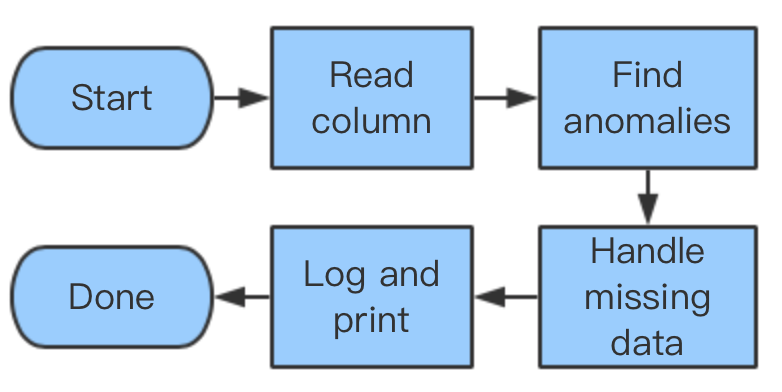
\includegraphics[width=3.8in]{flowchart.png}
\caption{The processing flowchar}\label{flowchart}
\end{figure}
%
\indent 1) For IP address, which is a categorical data, we figure out which type of IP a request is from. This is not easy to fill the missing and potentially wrong ones since we hardly have clues in the log file to rely on. So we can nothing towards them.
\\
\indent 2) For time, which is a numerical data, we correct errors like illegitimate time values. We fill the missing time value with the previous time, which is the easiest way to deal with the missing parts, for the log of the operations are in time order. Then we plot the distribution of requests with respect to time.
\\
\indent 3) For size, which is a numerical data, it is less possible to have extremely values, since people are accessing almost same type of files in regular size. So we replace anomalies and missing data with mean values.
\\
\indent 4) Apache HTTP code, which is a categorical data, represents the type of the response. We use the mode to fill the blank and then plot the distribution of different kinds of response because we are most likely to get similar responses.
\\
\indent 5) For using agent and crawler, which are categorical datas, we also use the mode to fill the missing data and plot the distribution of population using these techniques versus not. 
\\
\indent 6) For the browser field, which is a categorical data, we use the mode the fill the missing data. Then we plot the distribution of numbers of various browsers and get to the most-used browser. 
\\
%
\section{The package}\label{iii}
\indent Following the precessing idea in Sect. ~\ref{ii}, we develop this MissingData package in Python3 to finish the jobs stated above. The package takes into the year that is to be processed and automatically get the log files of first day of each month. After analysing, it upload all the data into an AWS S3 bucket.
\\
\indent The package can be divided into two modules, the preparation and the analysing module. The former dose log file URL generating according to the year provided. While the latter dose all the analysis work. Hear we focus on the analysing module and detail some implementations of the pipeline we build. 
\\
\indent 
%
\section{Result}\label{iv}
\indent The results of the concatenated data, metrics and logs are as follow:
\indent The final data, summary metric and log files are shown in Fig. ~\ref{data}.
\begin{figure}
\centering
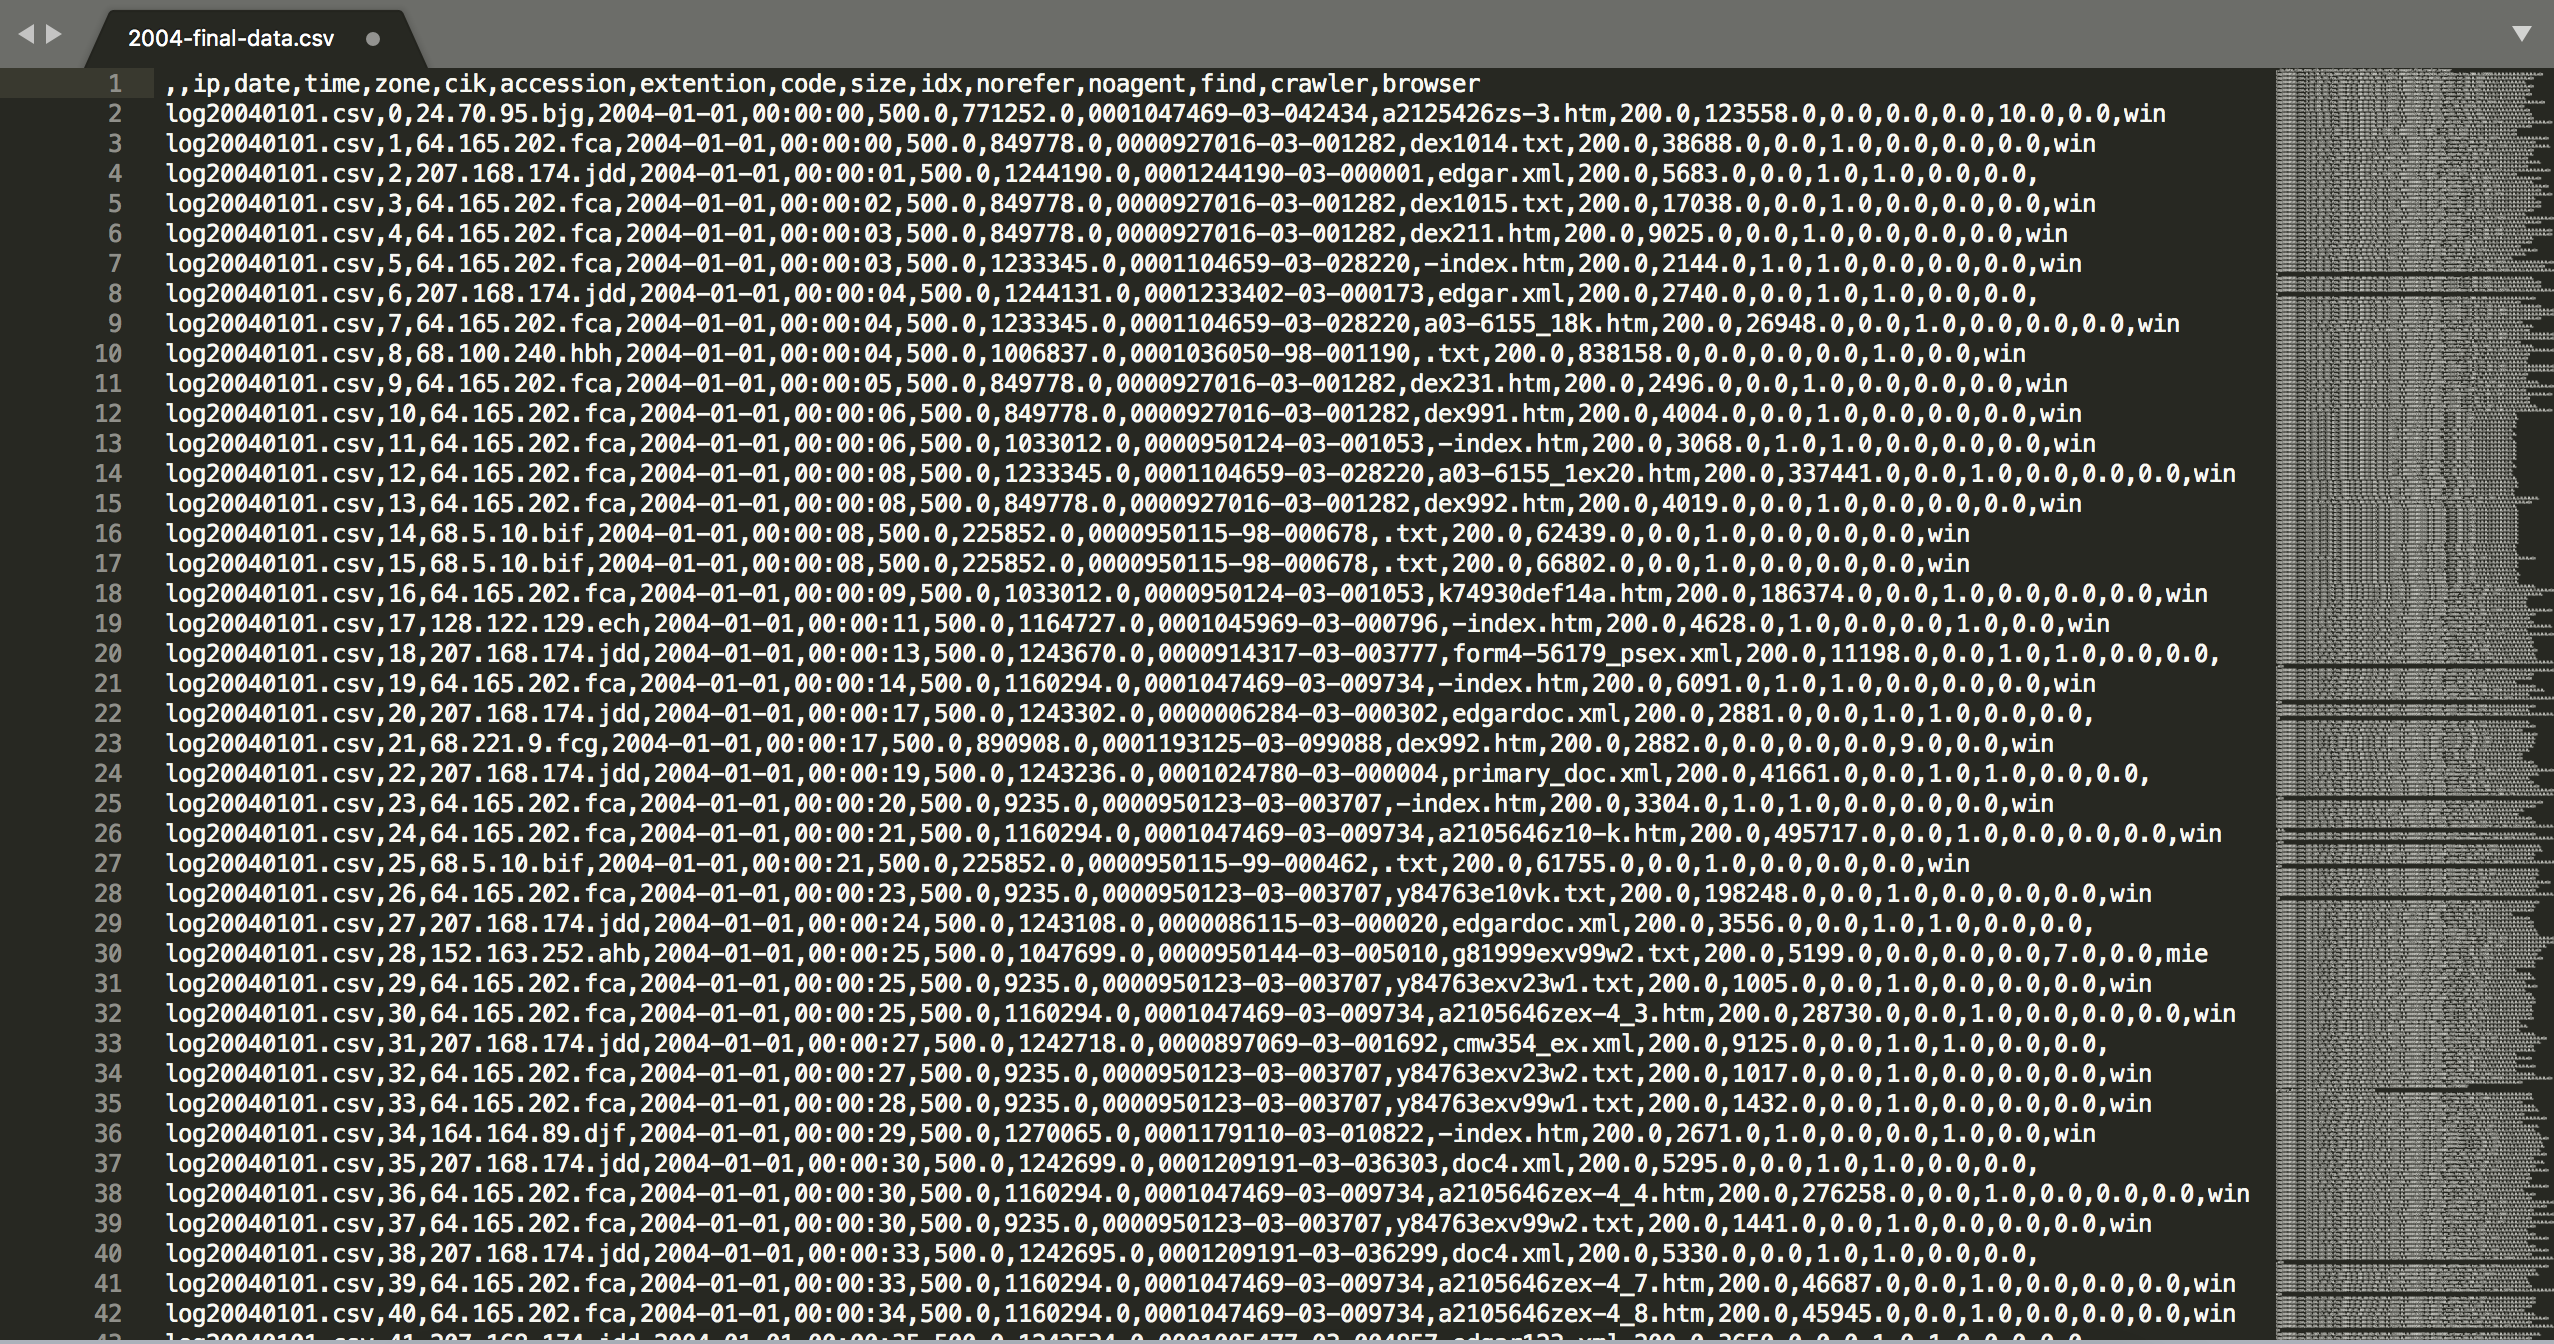
\includegraphics[width=3.6in]{final-data.png}
\caption{The flow diagram of the LCPR algorithm}\label{data}
\end{figure}
\begin{figure}
\centering
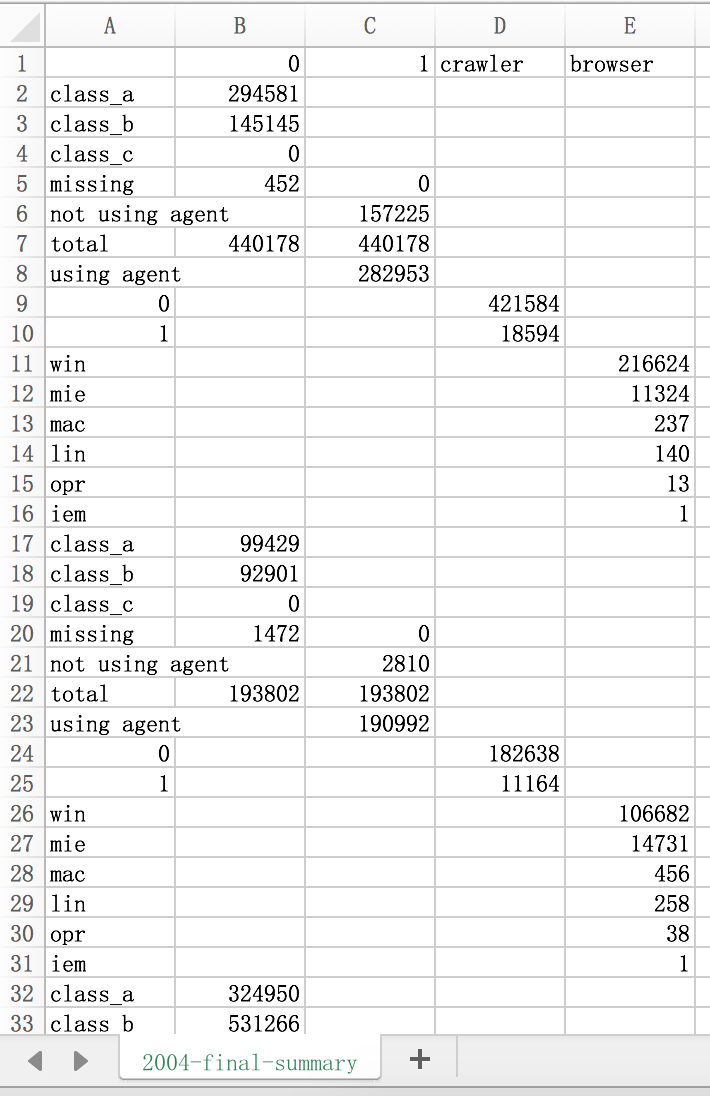
\includegraphics[width=3.6in]{final-sum.png}
\caption{The flow diagram of the LCPR algorithm}\label{sum}
\end{figure}
\begin{figure}
\centering
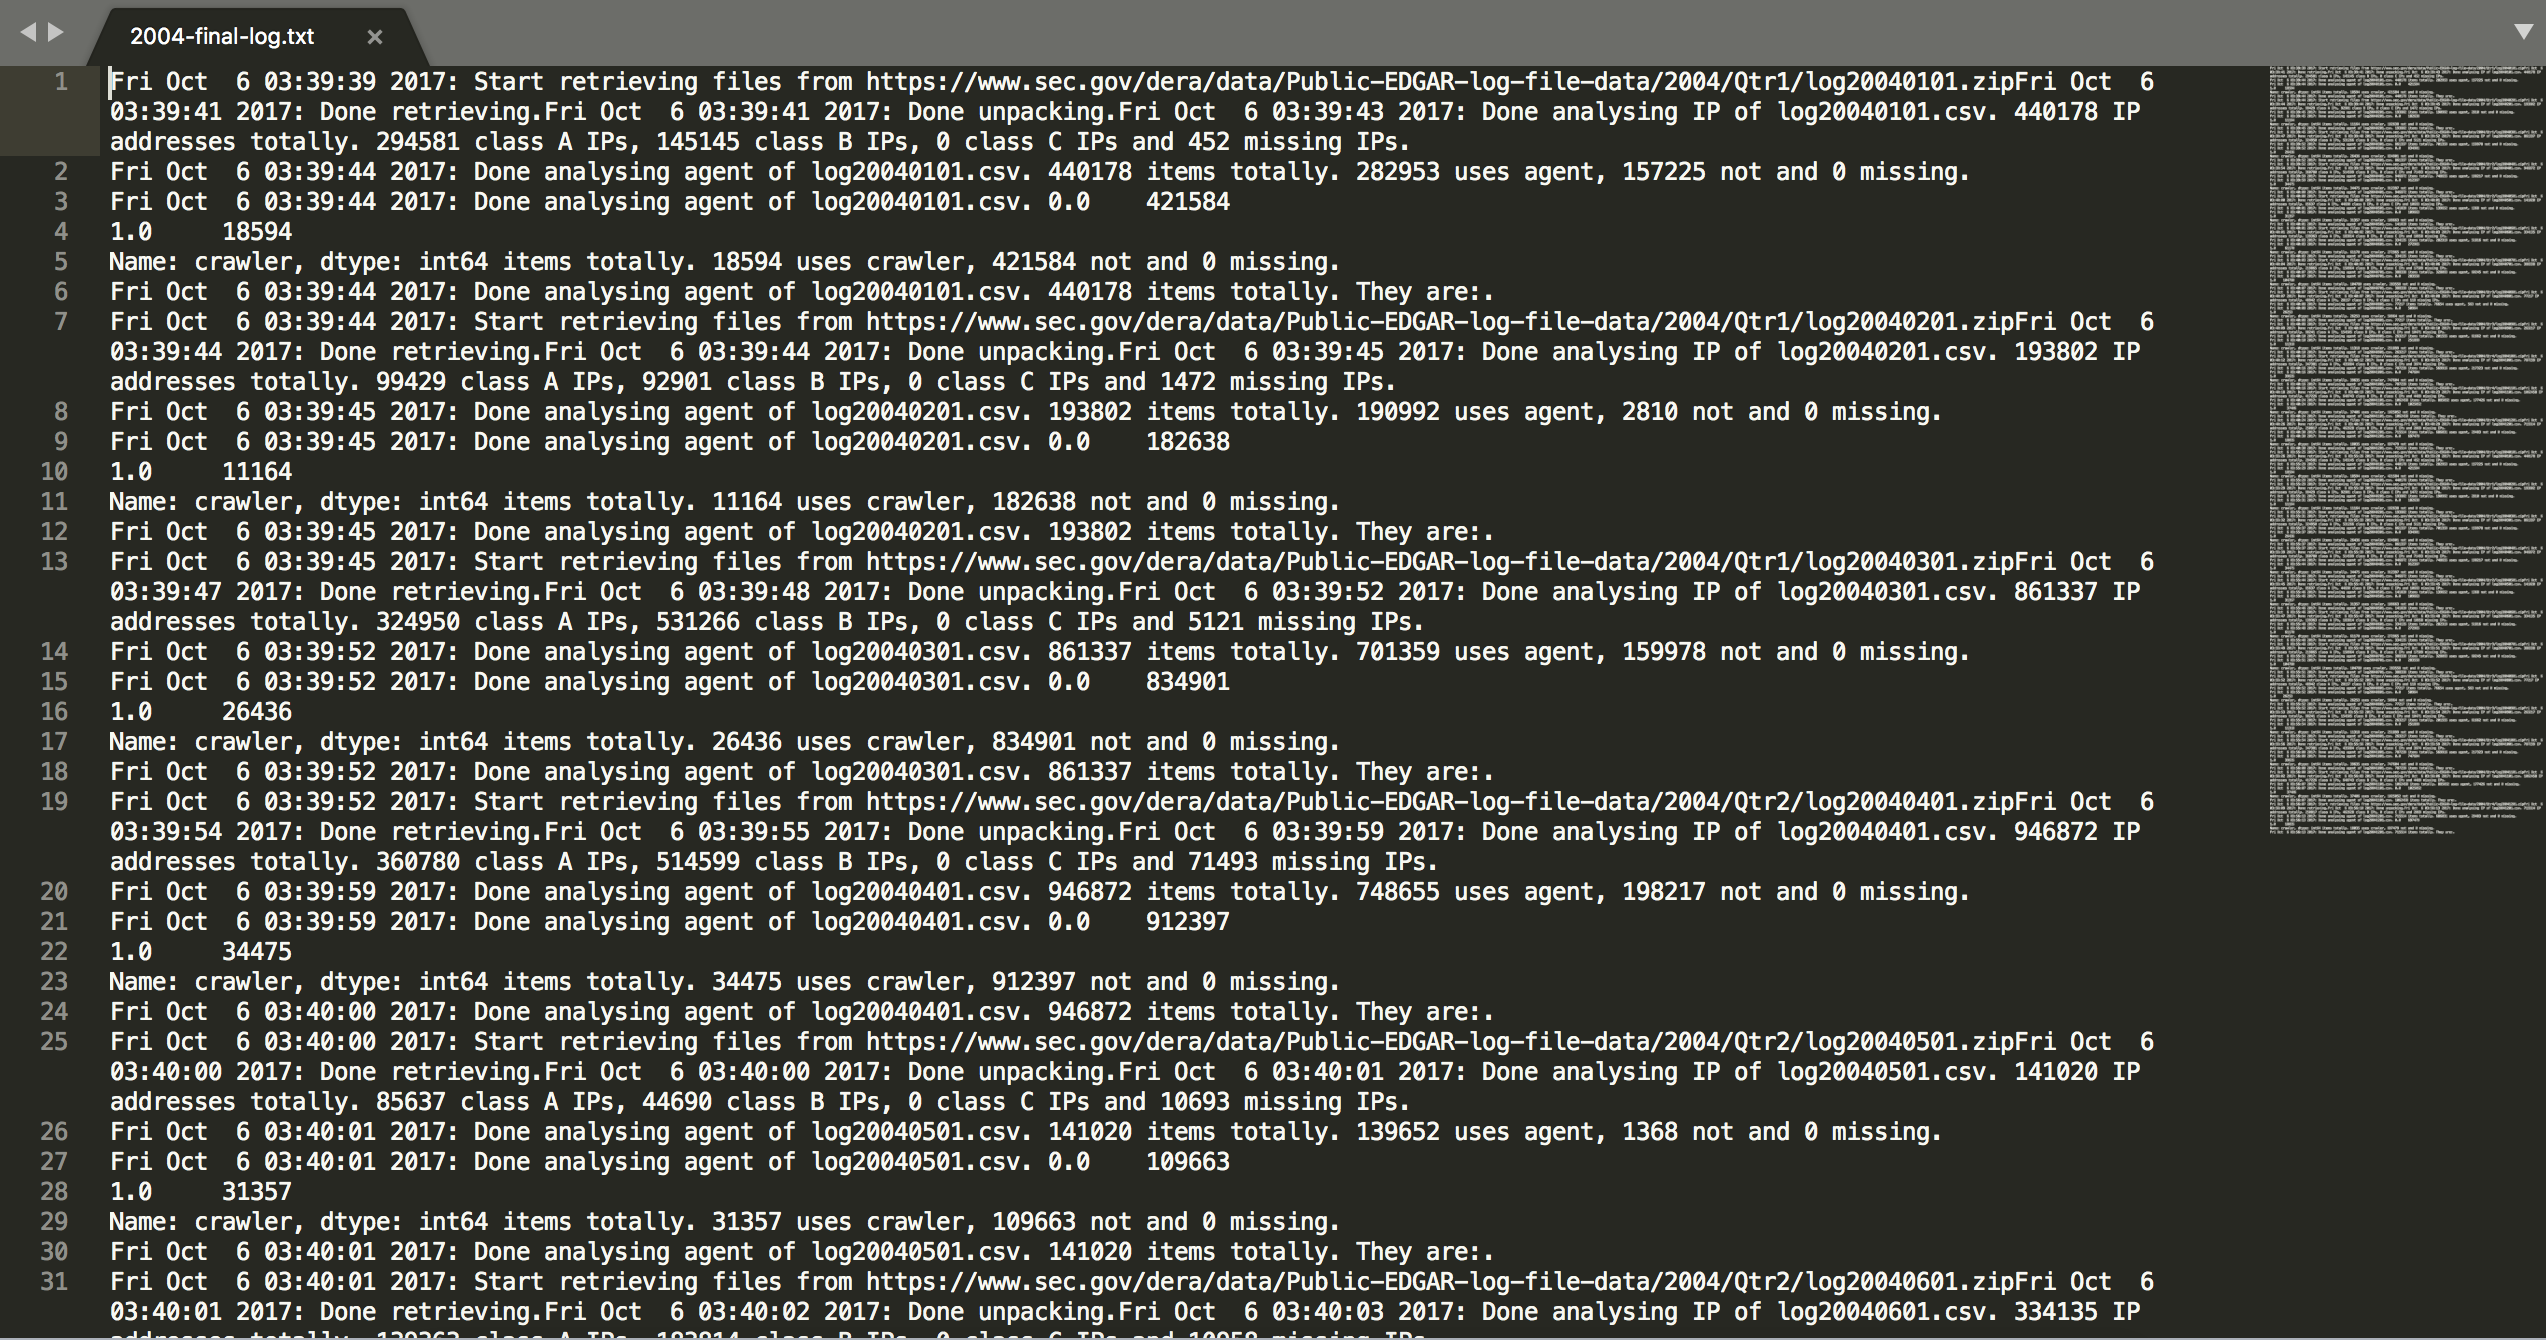
\includegraphics[width=3.6in]{final-log.png}
\caption{The flow diagram of the LCPR algorithm}\label{log}
\end{figure}
\indent In this paper, we analysed the EDGAR log files, in presence of missing and potentially wrong data item. Facing different field of data and different types of missing and anomalies, we adopt accordingly to find and correct the anomalies, as well as handling missing data. We retrieve log files from the EDGAR system, find anomalies, deal with missing data, compute metrics and upload useful information to AWS S3 bucket in Python3. Then we build a package to reuse this whole functionality and dockerize this pipeline to work in other environment.
\\
%
\begin{thebibliography}{1}
\bibitem
https://pandas.pydata.org/pandas-docs/stable/index.html
\bibitem{NASA's Space}
Chandola, V.; Banerjee, A.; Kumar, V. (2009). "Anomaly detection: A survey". ACM Computing Surveys. 41 (3): 1?58. doi:10.1145/1541880.1541882
\end{thebibliography}
\end{document} 